%% =====================================================================
%% IEEE CONFERENCE PAPER
%% Title : Interpretable and Uncertainty-Aware Crop Price Forecasting
%%         for Indian Markets using Temporal Fusion Transformers
%% Authors: Devulapalli Tharun, L. Preethi, Shashidhar G Koolagudi
%% File  : project_ieee_paper.tex
%% =====================================================================

\documentclass[conference,twoside]{IEEEtran}

\usepackage{cite}
\usepackage{amsmath,amssymb}
\usepackage{graphicx}
\usepackage{booktabs}
\usepackage{array}
\usepackage{url}
\usepackage[hidelinks]{hyperref}
\usepackage{xurl}
\usepackage{float}
\usepackage{xcolor}
\usepackage{tikz}
\usepackage{pgfplots}
\pgfplotsset{compat=1.18}
\usetikzlibrary{arrows.meta,positioning,shapes.geometric}

\title{Interpretable and Uncertainty-Aware Crop Price Forecasting
for Indian Markets using Temporal Fusion Transformers}

\author{
\IEEEauthorblockN{Devulapalli Tharun}
\IEEEauthorblockA{\textit{Dept. of Computer Science \& Engg.} \\
\textit{National Institute of Technology} \\
\textit{Surathkal, Karnataka, India} \\
\textit{devulapallitharun.252cs009@nitk.edu.in}}
\and
\IEEEauthorblockN{L. Preethi}
\IEEEauthorblockA{\textit{Dept. of Computer Science \& Engg.} \\
\textit{National Institute of Technology} \\
\textit{Surathkal, Karnataka, India} \\
\textit{preethi.237cs002@nitk.edu.in}}
\and
\IEEEauthorblockN{Shashidhar G Koolagudi}
\IEEEauthorblockA{\textit{Dept. of Computer Science \& Engg.} \\
\textit{National Institute of Technology} \\
\textit{Surathkal, Karnataka, India} \\
\textit{koolagudi@nitk.edu.in}}
}

\begin{document}
\maketitle

%% =====================================================================
%% ABSTRACT
%% =====================================================================
\begin{abstract}
Monthly retail food prices in India are difficult to forecast. A single number is rarely enough for a trader or a procurement officer to act on. A useful forecast must also give a range and some idea of what drives the prediction. This paper presents a system for three crops --- onions, tomatoes and rice --- that outputs a median forecast, a calibrated band, and a per-feature explanation for each of the next one to six months. Price data is taken from the WFP India retail panel. Weather data is taken from the NASA POWER monthly API.

XGBoost is used as the point baseline. A Temporal Fusion Transformer (TFT) is used for quantile forecasting. The XGBoost output is added as one of the known future inputs to TFT. Conformal Quantile Regression (CQR) then adjusts the $[q_{0.1}, q_{0.9}]$ band separately for each crop. The 2022 window is used as the calibration set.

On 792 test rows from January 2023 onward, the fused model gives 11.4 percent MAPE and 84.0 percent empirical band coverage. The paired $t$-test against a plain TFT gives $p = 4.6 \times 10^{-86}$, and Cohen's $d$ is $-0.79$. The Variable Selection Network ranking is stable across 1000 bootstrap resamples (Kendall $\tau = 0.942$). All artifacts are served through a Streamlit dashboard.
\end{abstract}

\begin{IEEEkeywords}
crop price forecasting, Temporal Fusion Transformer, probabilistic forecasting, conformal calibration, uncertainty quantification, agricultural market analytics
\end{IEEEkeywords}

%% =====================================================================
%% SECTION 1 — INTRODUCTION
%% =====================================================================
\section{Introduction}
\label{sec:introduction}

Food crop prices in India shift fast. Onion prices can move from around per kg Rs.\ 30 to Rs.\ 60 in a few months when the monsoon is late. Tomato prices in July 2023 climbed even higher. Such moves hit household food budgets, show up in retail inflation, and force the Food Corporation of India (FCI) to take buying and storage calls under real risk. In such a setting, a single forecast number is of limited use. A range of likely prices, with some idea of what drives the range, is far more useful.

Studies on Indian crop price forecasting have grown over the past decade. Nayak et al.\ \cite{nayak2024top} apply deep models with weather inputs to tomato, onion and potato prices. Manogna et al.\ \cite{manogna2025deep} compare LSTM, bidirectional RNN and gradient boosted tree models across many commodities. Paul et al.\ \cite{paul2022brinjal} work on brinjal prices. Two gaps are visible across these papers. The first is that every result is reported as a single point error such as MAPE or RMSE. The second is that none of these models exposes which input feature drove a particular prediction, which makes it hard to audit the forecast during a price spike.

The system in this paper closes both gaps for three crops. XGBoost is trained on the engineered lag, rolling and weather features and gives a strong point estimate. A Temporal Fusion Transformer (TFT) is trained on the same data and gives three quantile outputs per month: $q_{0.1}$, $q_{0.5}$ and $q_{0.9}$. The XGBoost output is added as one of the known future inputs to TFT, so the deep model can use it or discount it as required. Conformal Quantile Regression (CQR) then adjusts the band separately for each crop, using 2022 as the calibration year. The Variable Selection Network (VSN) weights from TFT are extracted and bootstrapped to show which features are consistently important.

On the January 2023 onward test period, the fused model reaches 11.4 percent MAPE and 84.0 percent empirical coverage across 792 test rows. The gain over a plain TFT is confirmed by a paired $t$-test ($p = 4.6 \times 10^{-86}$), a Wilcoxon test ($p = 1.2 \times 10^{-95}$), and a Cohen's $d$ of $-0.79$.

The rest of the paper is laid out as follows. Section~\ref{sec:contributions} states the contributions. Section~\ref{sec:literature} reviews related work by model family. Section~\ref{sec:dataset} describes the dataset. Section~\ref{sec:preprocessing} covers the feature engineering. Section~\ref{sec:methodology} describes the pipeline. Section~\ref{sec:results} reports the results with statistical validation. Section~\ref{sec:implementation} describes the dashboard. Section~\ref{sec:conclusion} closes with limitations and future work.

%% =====================================================================
%% SECTION 2 — CONTRIBUTIONS
%% =====================================================================
\section{Contributions}
\label{sec:contributions}

The system differs from the reviewed literature in four concrete ways.

\textbf{1.\ XGBoost output used as a TFT input.} An XGBoost model is trained on data up to 2019 only. Its log-price predictions are then computed for the full timeline and attached as a known future input to TFT. TFT's Variable Selection Network then decides at each time step how much weight to give this signal. This is not model stacking \cite{wolpert1992stacking}, where two models predict independently and results are merged afterward. Instead, the tree-model output enters TFT as just another feature — one the network can trust or ignore depending on the context. For rice, whose prices are stable and well-predicted by lag features, the XGBoost signal tends to get high weight. For tomatoes during a heat spike, where the tree model can seriously underestimate because it cannot extrapolate to price levels it has not seen, TFT can reduce that weight and rely more on its sequential history. The 2019 cutoff is deliberate: it keeps the auxiliary model from seeing any 2022 or 2023 data, so the CQR calibration window remains uncontaminated.

\textbf{2.\ CQR applied per crop on log-price residuals.} Conformal Quantile Regression \cite{romano2019cqr} is applied separately to each crop on the 2022 validation window, working in log-price space. Fitting a single global offset across all three crops does not work here. The offset that brings rice coverage to the right level leaves the tomato band far too narrow, since tomato prices can double in a single month while rice prices barely shift.

\textbf{3.\ Every accuracy claim is backed by three tests.} The improvement over plain TFT is checked with a paired $t$-test, a Wilcoxon signed-rank test and Cohen's $d$, on the same $n = 792$ matched test rows. The $t$-test checks the mean error difference directly. The Wilcoxon test provides a non-parametric check that does not assume normality of residuals. Cohen's $d$ guards against the possibility that a large sample size alone makes a tiny improvement look significant — a value of $|d| > 0.5$ is needed to call the gain practically meaningful. Empirical coverage is tested separately per crop against the nominal 80 percent target using an exact binomial test. The VSN feature ranking is checked across 1000 bootstrap resamples using pairwise Kendall $\tau$.

\textbf{4.\ A working dashboard.} The trained artifacts load into a Streamlit application. A procurement officer can open it, select a crop and market, and get a six-month forecast with a calibrated price band and a risk label, without running any scripts. Three supporting views show the price history with model overlay, the VSN and attention-based explanations, and a test-validation view on 2023 actual data.

%% =====================================================================
%% SECTION 3 — LITERATURE REVIEW
%% =====================================================================
\section{Literature Review}
\label{sec:literature}

Indian crop price forecasting has been approached with a range of models, from classical time-series methods to deep learning architectures.

\subsection{Statistical and Classical Methods}
ARIMA and SARIMA remain the most commonly cited baselines for monthly agricultural price series \cite{box2015arima}. Their appeal is transparency: the differencing order and seasonal structure are set explicitly, and the model assumptions can be written down. The problem shows up during price spikes. A model built on the assumption that the series reverts after differencing does not have a natural way to handle a non-linear event like the late-2019 onion shortage or the mid-2023 tomato surge. Adding weather as an external regressor is possible but requires the lag structure to be specified manually rather than learned from data.

\subsection{Machine Learning Methods}
Tree-based methods --- Random Forest, XGBoost, Support Vector Regression --- are consistently more accurate than ARIMA on engineered tabular features that include lags and rolling means. Manogna et al.\ \cite{manogna2025deep} demonstrate this pattern across several Indian commodities. The issue with these models is not their point accuracy. It is that the output is a single value. SHAP and gain-based feature importances summarise the whole training set; they cannot say which variable drove the prediction for the specific month when onion prices crossed Rs.\ 100. There is also no native mechanism to produce an interval.

\subsection{Recurrent Deep Learning Methods}
LSTM and GRU networks handle sequential price dependence more naturally than tabular methods and take exogenous weather or calendar inputs without manual lag specification. Nayak et al.\ \cite{nayak2024top} and Paul et al.\ \cite{paul2022brinjal} report competitive results on Indian crop prices with these architectures. The uncertainty quantification step is usually bolted on: either retrain with quantile loss or add Monte Carlo dropout. Neither approach produces a band with a tested coverage guarantee.

\subsection{Transformer-Based and Attention Methods}
Probabilistic deep forecasters have expanded rapidly. DeepAR \cite{salinas2020deepar} models the full predictive distribution through parametric output heads. Informer \cite{zhou2021informer}, N-BEATS \cite{oreshkin2020nbeats}, NHITS \cite{challu2023nhits} and PatchTST \cite{nie2023patchtst} target long horizons through sparse attention or learned decompositions. The M4 and M5 forecasting competitions \cite{makridakis2018m4, makridakis2022m5accuracy, makridakis2022m5uncertainty} and the empirical study by Zeng et al.\ \cite{zeng2023transformers} suggest no single architecture is best across settings; the right choice depends on sequence length, covariate structure and whether the application needs interpretable outputs. TFT \cite{lim2021tft} was chosen here specifically because it handles mixed static and time-varying inputs, produces multi-horizon quantile forecasts natively, and exposes per-timestep input weights through its Variable Selection Network --- all three of which are required for this application.

The gap specific to Indian crop price forecasting is that no reviewed study produces all of: a calibrated band with empirically tested coverage, a feature ranking validated against resampling noise, and a working interface. Most studies report a single point-error number and stop there. In the present work, the tree model's strength on tabular features is preserved by feeding XGBoost output back into TFT as a known input, and CQR is applied per crop so that the band stays reliable. Table~\ref{tab:lit_summary} summarises this positioning.

\begin{table*}[!t]
\centering
\caption{Summary of literature groups and what each leaves open. ``Calibrated band'' means the prediction interval has been empirically tested for coverage. ``Stable explanation'' means the feature ranking has been validated across resamples.}
\label{tab:lit_summary}
\begin{tabular}{p{4.2cm}cccc}
\toprule
\textbf{Method group} & \textbf{Point accuracy} & \textbf{Calibrated band} & \textbf{Stable explanation} & \textbf{Deployed dashboard} \\
\midrule
Statistical (ARIMA, SARIMA)          & moderate & no  & no & no \\
ML (RF, XGBoost, SVR)                & strong   & no  & partial (static) & rare \\
Recurrent (LSTM, GRU)                & strong   & rare & no & rare \\
Transformer (DeepAR, TFT, Informer)  & strong   & sometimes & partial & rare \\
\textbf{This work}                   & \textbf{strong} & \textbf{yes (tested)} & \textbf{yes (bootstrap)} & \textbf{yes} \\
\bottomrule
\end{tabular}
\end{table*}

%% =====================================================================
%% SECTION 4 — DATASET
%% =====================================================================
\section{Dataset}
\label{sec:dataset}

\subsection{Data Sources}
Three public sources of Indian crop price data were evaluated. Agmarknet, run by the Government of India, has daily mandi-level wholesale prices for many crops. However, market coverage is patchy across states, and a wholesale-to-retail mapping would introduce extra error. The Department of Consumer Affairs daily retail panel is closer to the target, but the historical depth is short --- a few years for most cities --- which is not enough for a model with a 24-month encoder window. The WFP India retail dataset \cite{wfp2026dataset} was chosen instead. It has monthly retail prices from 1994 onward across more than a hundred markets, with a consistent schema across years. The monthly granularity matches realistic planning horizons. The long history covers the 2008 food price shock, the 2014--15 onion spike and the COVID disruption, all in the training window.

For weather, Indian ground station data has gaps in rural market locations. The NASA POWER monthly point API \cite{nasa2026power} gives satellite-derived monthly estimates at any latitude-longitude pair with no missing values. This makes it practical to match weather to all 53 markets in the panel. Three variables are used: monthly total rainfall, mean temperature and mean relative humidity. These three directly affect vegetable yield during growing and transport.

\subsection{Dataset Preparation}
The raw WFP file has 145{,}124 rows covering 41 commodities, 170 markets and the years 1994 onward. This is filtered down in a few steps to reach the panel used for modeling. Each step in Table~\ref{tab:filtering} corresponds to one constraint imposed by the modeling pipeline: keeping only retail records (the wholesale series is a different formation process), keeping only KG units (so the price target is comparable across rows), dropping aggregate national records (they are not real market locations), keeping only the three commodities of interest, dropping series shorter than 60 months (TFT needs 24 encoder months plus several training windows), and forward-filling short internal gaps to keep the monthly grid regular.

\begin{table*}[!t]
\centering
\caption{Step-by-step filtering of the raw WFP India dataset. Each row removes one type of record and states why that removal is needed for the modeling pipeline.}
\label{tab:filtering}
\begin{tabular}{p{0.5cm}p{4.5cm}cp{8.5cm}}
\toprule
\textbf{\#} & \textbf{Filter step} & \textbf{Rows after} & \textbf{Why the step is needed} \\
\midrule
0 & Raw WFP India price data         & 145{,}124 & starting point before any filtering \\
1 & Keep retail records only         & 90{,}312  & wholesale and farm-gate prices follow a different formation process and should not be mixed with retail \\
2 & Keep KG unit only                & 87{,}501  & a few rows use liters or 100g; mixing units would corrupt the price target \\
3 & Drop national and aggregate records & 84{,}920  & rows tagged ``National Average'' and similar are not real market locations and break the per-market structure \\
4 & Keep onions, tomatoes, rice only & 21{,}458  & three commodities chosen to span low, medium and high price volatility (Section~\ref{sec:why_three}) \\
5 & Drop series with $<$60 months    & 17{,}812  & TFT needs at least 24 encoder months plus enough training windows; very short series cannot be used \\
6 & Forward-fill short internal gaps & 16{,}939  & keeps a regular monthly panel without imputing across long missing runs \\
\bottomrule
\end{tabular}
\end{table*}

The resulting panel has 16{,}939 monthly observations across 123 market-crop series in 53 markets, covering January 1995 to July 2023.

\subsection{Crop Selection}
\label{sec:why_three}
The three crops were picked to span a wide range of price behaviour. Volatility is measured here by the Coefficient of Variation (CV): standard deviation divided by mean, expressed as a percentage.

\begin{itemize}
    \item \textbf{Onions} have a CV of about 60 percent. The kharif and rabi cycles and storage losses make prices volatile. The price episode of late 2019, when retail onion prices climbed sharply, sits in the training window.
    \item \textbf{Tomatoes} have a CV of about 90 percent and are the most volatile of the three. Prices are very sensitive to short-duration heat and rain events. The mid-2023 price episode sits in the test period.
    \item \textbf{Rice} has a CV of about 20 percent and is the most stable, supported by government procurement and the public distribution system. Rice acts as a low-volatility reference: a model that does well on rice but poorly on tomatoes is mostly picking up easy patterns.
\end{itemize}

\subsection{Temporal Split}
A strict chronological split is used throughout so that no future data leaks into training. Table~\ref{tab:split} shows the calendar split. A random split would let 2023 months appear in the training set and inflate the test accuracy, which a deployed forecaster cannot do.

\begin{table}[H]
\centering
\caption{Time-based split used for the final model. The 2022 window doubles as the calibration set for CQR. The test period is the held-out 2023 onward data that the model never sees during training or calibration.}
\label{tab:split}
\begin{tabular}{lccc}
\toprule
\textbf{Split} & \textbf{Date range} & \textbf{Rows} & \textbf{Series} \\
\midrule
Train                  & up to 31 Dec 2021        & 14{,}686 & 123 \\
Validation--calibration & 1 Jan -- 31 Dec 2022      & 1{,}461  & 123 \\
Test                   & 1 Jan 2023 onward        & 792      & 123 \\
\bottomrule
\end{tabular}
\end{table}

%% =====================================================================
%% SECTION 5 — FEATURE ENGINEERING
%% =====================================================================
\section{Feature Engineering}
\label{sec:preprocessing}

Index $s$ denotes one market-crop series (e.g., onions in Bangalore, rice in Hyderabad) and $t$ is the month. $p_{s,t}$ is the retail price in Rs.\ per kg. All features below are computed from the same raw columns and shared by both XGBoost and TFT.

\subsection{Log transform on the target price}
\begin{equation}
y_{s,t} = \log(1 + p_{s,t})
\label{eq:logtransform}
\end{equation}
The $+1$ shift handles zero-price rows. In log space a tomato spike from per kg Rs.\ 40 to Rs.\ 120 has the same magnitude as a move from Rs.\ 10 to Rs.\ 30 --- the model is not disproportionately pulled by high-price months. Inverse transform to recover price scale:
\begin{equation}
\hat{p}_{s,t} = \exp(\hat{y}_{s,t}) - 1
\label{eq:invlog}
\end{equation}

\subsection{Lag features}
\begin{align}
\text{lag}_{1}(s,t)  &= p_{s,t-1} \label{eq:lag1}\\
\text{lag}_{12}(s,t) &= p_{s,t-12} \label{eq:lag12}
\end{align}
The one-month lag carries short-run momentum. The twelve-month lag gives the model a direct look at the same seasonal window from the previous year, which is particularly useful for onions where kharif and rabi harvest timing repeats annually.

\subsection{Rolling means}
\begin{align}
\text{roll}_{3}(s,t) &= \tfrac{1}{3}\textstyle\sum_{k=0}^{2} p_{s,t-k} \label{eq:roll3}\\
\text{roll}_{6}(s,t) &= \tfrac{1}{6}\textstyle\sum_{k=0}^{5} p_{s,t-k} \label{eq:roll6}
\end{align}
The three-month window captures the recent trend without overreacting to a single outlier month. The six-month window gives a slower-moving baseline, so the model can distinguish a brief spike from a genuine regime change in the local price level.

\subsection{Year-on-year change}
\begin{equation}
\text{yoy\_change}(s,t) = \frac{p_{s,t} - p_{s,t-12}}{p_{s,t-12}}
\label{eq:yoy}
\end{equation}
This fraction tells the model whether the current month is running ahead of or behind the same seasonal window last year, which is more informative than the raw lag value alone.

\subsection{Cyclical month encoding}
\begin{align}
m_{\sin}(t) &= \sin\!\Bigl(\tfrac{2\pi\,\text{month}(t)}{12}\Bigr) \label{eq:msin}\\
m_{\cos}(t) &= \cos\!\Bigl(\tfrac{2\pi\,\text{month}(t)}{12}\Bigr) \label{eq:mcos}
\end{align}
Integer month encoding creates a false discontinuity between December (12) and January (1), which are in fact adjacent in the annual cycle. The sine-cosine pair wraps the month onto a unit circle, so the model sees December and January as neighbours.

\subsection{Weather shock binary flags}
\begin{align}
\text{rain\_deficit}(s,t)  &= \mathbf{1}\!\left[\text{rainfall}(s,t) < 50\,\text{mm}\right] \label{eq:rain_def}\\
\text{rain\_excess}(s,t)   &= \mathbf{1}\!\left[\text{rainfall}(s,t) > 300\,\text{mm}\right] \label{eq:rain_exc}\\
\text{heat\_stress}(s,t)   &= \mathbf{1}\!\left[\text{temp\_mean}(s,t) > 38^{\circ}\text{C}\right] \label{eq:heat}\\
\text{cold\_stress}(s,t)   &= \mathbf{1}\!\left[\text{temp\_mean}(s,t) < 5^{\circ}\text{C}\right] \label{eq:cold}
\end{align}
The 50 mm deficit threshold is roughly half the long-run monthly average for the non-monsoon belt, around the agronomic point where vegetable crops show measurable water stress. At 300 mm excess, standing crops in low-lying fields begin to flood. The 38$^\circ$C heat flag covers the temperature range known to cause fruit drop in tomatoes; the 5$^\circ$C cold flag picks up north Indian winter months when cold damage affects rabi onion and tomato crops. Encoding these as binary flags rather than using the raw continuous value makes it easier for the model to fire a strong response at the threshold rather than trying to interpolate through it.

\subsection{COVID lockdown flag}
\begin{equation}
\text{covid\_lockdown}(t) = \mathbf{1}\!\left[t \in [\text{March 2020}, \text{June 2021}]\right]
\label{eq:covid}
\end{equation}
This flag marks the lockdown period so that the model does not generalise from the broken supply chains and irregular trading of that period to normal months.

\subsection{Final feature schema}
Table~\ref{tab:features} groups the resulting features by type. The fusion signal $xgb\_log\_pred$ is described in Section~\ref{sec:fusion} and is added only for the final model.

\begin{table*}[!t]
\centering
\caption{Features used for modeling, grouped by type. The fusion signal is added only for the final model.}
\label{tab:features}
\begin{tabular}{p{3.2cm}p{13.0cm}}
\toprule
\textbf{Group} & \textbf{Variables} \\
\midrule
Static descriptors  & commodity, market, state \\
Calendar / season   & month, year, month\_sin, month\_cos, agricultural season \\
Price memory        & price\_lag\_1m, price\_lag\_12m, rolling\_3m, rolling\_6m, yoy\_change \\
Weather (continuous)& rainfall\_monthly, temperature\_mean, humidity\_mean \\
Weather shock flags & rain\_deficit, rain\_excess, heat\_stress, cold\_stress \\
Event flag          & covid\_lockdown \\
Fusion signal       & xgb\_log\_pred (final model only) \\
\bottomrule
\end{tabular}
\end{table*}

%% =====================================================================
%% SECTION 6 — METHODOLOGY
%% =====================================================================
\section{Methodology}
\label{sec:methodology}

The pipeline has three stages. XGBoost takes the engineered features and outputs a point log-price estimate. TFT takes that estimate as one of its known future inputs and outputs three quantile forecasts per month: a lower bound, a median and an upper bound. Per-crop CQR then adjusts the interval on the 2022 calibration window so the target coverage holds on unseen data. Fig.~\ref{fig:pipeline_overview} shows how the stages connect.

\begin{figure}[t]
\centering
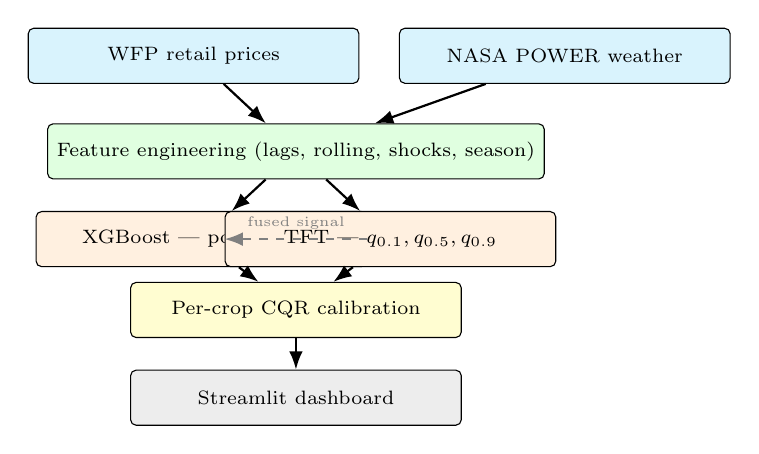
\begin{tikzpicture}[
  node distance=4mm,
  block/.style={draw, rounded corners=2pt, align=center, font=\scriptsize,
                minimum width=42mm, minimum height=7mm, fill=white},
  data/.style ={block, fill=cyan!15},
  proc/.style ={block, fill=green!12},
  model/.style={block, fill=orange!12},
  cal/.style  ={block, fill=yellow!18},
  ui/.style   ={block, fill=gray!14},
  arr/.style  ={-Latex, thick}
]
\node[data]  (d1)   {WFP retail prices};
\node[data,  right=5mm of d1] (d2) {NASA POWER weather};
\node[proc,  below=5mm of d1, xshift=13mm] (feat)
      {Feature engineering (lags, rolling, shocks, season)};
\node[model, below=4mm of feat, xshift=-12mm] (xgb)
      {XGBoost --- point signal};
\node[model, below=4mm of feat, xshift=12mm] (tft)
      {TFT --- $q_{0.1},q_{0.5},q_{0.9}$};
\node[cal,   below=13mm of feat] (cqr)
      {Per-crop CQR calibration};
\node[ui,    below=4mm of cqr]  (ui)
      {Streamlit dashboard};
\draw[arr] (d1)   -- (feat);
\draw[arr] (d2)   -- (feat);
\draw[arr] (feat) -- (xgb);
\draw[arr] (feat) -- (tft);
\draw[arr] (xgb)  -- (cqr);
\draw[arr] (tft)  -- (cqr);
\draw[arr,dashed,gray] (xgb.east) -- node[above,font=\tiny]{fused signal} (tft.west);
\draw[arr] (cqr)  -- (ui);
\end{tikzpicture}
\caption{Pipeline overview. WFP prices and NASA POWER weather feed shared feature engineering. XGBoost produces a point prediction that is injected into TFT as a known covariate (dashed arrow). TFT outputs three quantile predictions. Per-crop CQR adjusts the band. All artifacts load into the dashboard.}
\label{fig:pipeline_overview}
\end{figure}

\begin{figure*}[t]
\centering
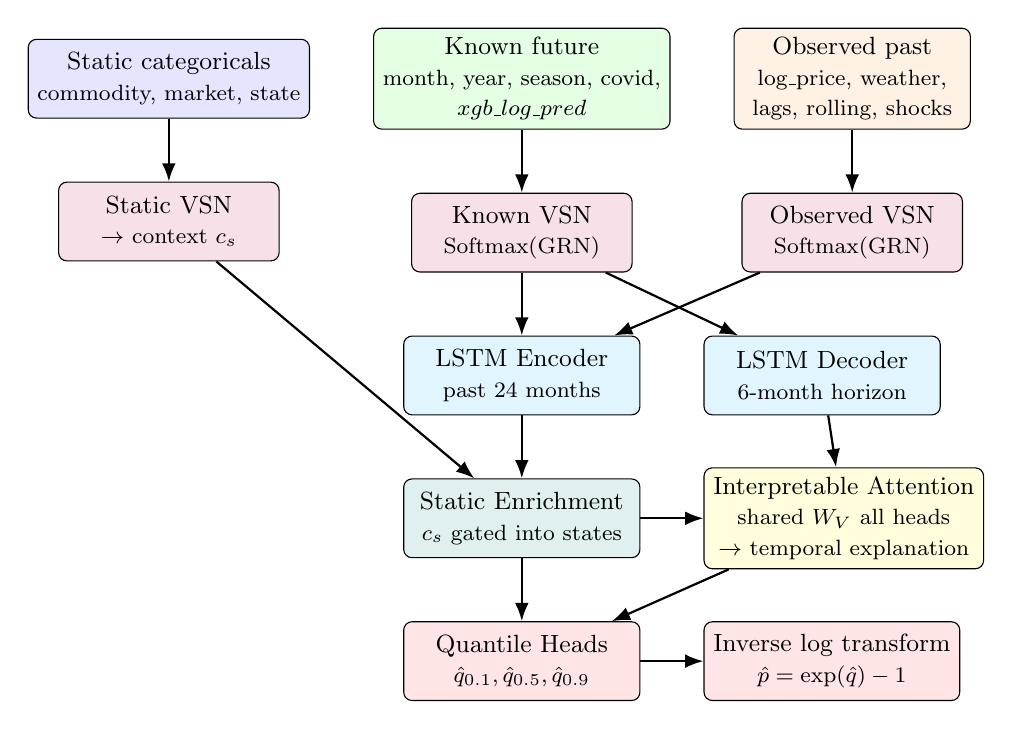
\begin{tikzpicture}[
  node distance=5mm,
  font=\small,
  box/.style={draw, rounded corners=3pt, align=center,
              minimum height=10mm, minimum width=30mm, fill=white},
  inp/.style ={box, fill=blue!10},
  vsn/.style ={box, fill=purple!12, minimum width=28mm},
  lstm/.style={box, fill=cyan!12,   minimum width=30mm},
  se/.style  ={box, fill=teal!12,   minimum width=30mm},
  attn/.style={box, fill=yellow!14, minimum width=35mm},
  qout/.style={box, fill=red!10,    minimum width=30mm},
  arr/.style ={-Latex, thick}
]

\node[inp, fill=blue!10]    (si)  {Static categoricals\\{\footnotesize commodity, market, state}};
\node[inp, fill=green!10, right=8mm of si] (ki)
      {Known future\\{\footnotesize month, year, season, covid,}\\{\footnotesize $xgb\_log\_pred$}};
\node[inp, fill=orange!10, right=8mm of ki] (oi)
      {Observed past\\{\footnotesize log\_price, weather,}\\{\footnotesize lags, rolling, shocks}};

\node[vsn, below=8mm of si] (vsn_s)
      {Static VSN\\{\footnotesize $\rightarrow$ context $c_s$}};
\node[vsn, below=8mm of ki] (vsn_k)
      {Known VSN\\{\footnotesize Softmax(GRN)}};
\node[vsn, below=8mm of oi] (vsn_o)
      {Observed VSN\\{\footnotesize Softmax(GRN)}};

\node[lstm, below=8mm of vsn_k] (enc)
      {LSTM Encoder\\{\footnotesize past 24 months}};
\node[lstm, right=8mm of enc] (dec)
      {LSTM Decoder\\{\footnotesize 6-month horizon}};

\node[se,   below=8mm of enc]   (se)  {Static Enrichment\\{\footnotesize $c_s$ gated into states}};
\node[attn, right=8mm of se]    (mha)
      {Interpretable Attention\\{\footnotesize shared $W_V$ all heads}\\{\footnotesize $\rightarrow$ temporal explanation}};

\node[qout, below=8mm of se]    (qh)
      {Quantile Heads\\{\footnotesize $\hat{q}_{0.1},\hat{q}_{0.5},\hat{q}_{0.9}$}};
\node[qout, right=8mm of qh]    (inv)
      {Inverse log transform\\{\footnotesize $\hat{p}=\exp(\hat{q})-1$}};

\draw[arr] (si)    -- (vsn_s);
\draw[arr] (ki)    -- (vsn_k);
\draw[arr] (oi)    -- (vsn_o);
\draw[arr] (vsn_s) -- (se);
\draw[arr] (vsn_k) -- (enc);
\draw[arr] (vsn_o) -- (enc);
\draw[arr] (vsn_k) -- (dec);
\draw[arr] (enc)   -- (se);
\draw[arr] (dec)   -- (mha);
\draw[arr] (se)    -- (mha);
\draw[arr] (se)    -- (qh);
\draw[arr] (mha)   -- (qh);
\draw[arr] (qh)    -- (inv);
\end{tikzpicture}
\caption{TFT architecture. Three input streams --- static categoricals (blue), known future covariates (green), and observed historical values (orange) --- each pass through a Variable Selection Network (VSN, purple) that computes per-timestep input weights via a Softmax-weighted Gated Residual Network (GRN). Weighted inputs feed an LSTM encoder (past 24 months) and decoder (6-month horizon). A static enrichment gate injects market-crop context ($c_s$) into the LSTM states. An interpretable multi-head attention layer with shared value projection $W_V$ attends over encoder history to produce temporal explanation weights. Three quantile heads output $\hat{q}_{0.1},\hat{q}_{0.5},\hat{q}_{0.9}$ per future step. An inverse log transform converts predictions back to price scale.}
\label{fig:tft_architecture}
\end{figure*}

\subsection{XGBoost baseline}
XGBoost \cite{chen2016xgboost} is a gradient boosted decision tree ensemble that grows trees sequentially, each new tree trained to reduce the residual error of the previous ones. It is used as the point baseline because tree ensembles are effective on tabular features with lags, rolling means and weather columns, and are robust to outliers and missing values. The model is trained on the engineered feature set (Table~\ref{tab:features}, without the fusion signal) to predict the log price for the next month.

Hyperparameters and rationale:
\begin{itemize}
    \item learning\_rate $= 0.05$: small enough that each tree only nudges the ensemble, large enough that 500 rounds is sufficient for convergence.
    \item max\_depth $= 6$: captures interactions between weather, season and lag features without overfitting on this dataset size.
    \item n\_estimators $= 500$ with early stopping on validation MAE: stops adding trees once validation error stops improving.
    \item objective = \texttt{reg:squarederror}: standard squared-error regression loss for log price prediction.
\end{itemize}

\subsection{Temporal Fusion Transformer (TFT)}
TFT \cite{lim2021tft} is a deep neural network for multi-horizon forecasting. It takes a window of past months, known future values such as calendar position and seasonal flags, and static descriptors of the series, and produces a prediction for each future month of the horizon. Three components separate it from a plain LSTM: a Variable Selection Network that learns which inputs matter at each time step, a static enrichment layer that carries market-crop context through the whole network, and quantile output heads that produce three predictions per step rather than one.

\textbf{Inputs.} Static categorical inputs include crop type, market name and state, embedded into a vector shared across all time steps for that series. Time-varying known inputs are values whose future is available at prediction time: year, month, cyclically encoded month, agricultural season, the COVID lockdown flag, and in the final model the fused XGBoost prediction. Time-varying observed inputs are values whose future is unknown but past is observed: log price, rainfall, temperature, humidity, lag and rolling features, and weather shock flags.

\textbf{Variable Selection Network (VSN).} For each time step $t$, VSN computes a Softmax weight over all available inputs $X_t$ given the static context $c_s$:
\begin{equation}
v_t = \mathrm{Softmax}\!\left( \mathrm{GRN}(X_t, c_s) \right)
\label{eq:vsn}
\end{equation}
GRN is a Gated Residual Network, a two-layer feed-forward block with a gated linear unit and a residual connection. The weight $v_t$ indicates how much each input contributes at that time step and is exposed to the user as the explanation signal.

\textbf{LSTM encoder-decoder.} Past time steps pass through an LSTM encoder and the future horizon through an LSTM decoder, giving the model sequential context around the forecast.

\textbf{Interpretable multi-head attention.} A self-attention layer attends over the encoder output. TFT uses a simplified design that shares the value projection $W_V$ across all attention heads, so head-averaged attention weights directly indicate which past months were most relevant for the current forecast.

\textbf{Quantile heads.} The decoder produces three predictions per future month: $\hat{q}_{0.1}$, $\hat{q}_{0.5}$ and $\hat{q}_{0.9}$. They are trained jointly using the pinball loss:
\begin{equation}
\rho_{\tau}(y, \hat{q}_\tau) =
\begin{cases}
\tau \cdot (y - \hat{q}_\tau), & y \geq \hat{q}_\tau \\
(1-\tau) \cdot (\hat{q}_\tau - y), & y < \hat{q}_\tau
\end{cases}
\label{eq:pinball}
\end{equation}
For $\tau = 0.5$ the pinball loss reduces to absolute error, giving the median prediction. For $\tau = 0.1$ it penalises over-prediction nine times more than under-prediction, which pushes the head to produce a low estimate. For $\tau = 0.9$ it does the opposite.

Hyperparameters were chosen to match the dataset size of 16{,}939 rows:
\begin{itemize}
    \item hidden\_size $= 32$, hidden\_continuous\_size $= 16$: kept small to avoid overfitting.
    \item lstm\_layers $= 1$, attention\_head\_size $= 2$: minimal depth for monthly data.
    \item dropout $= 0.2$: standard regularisation.
    \item learning\_rate $= 0.03$, batch\_size $= 64$.
    \item max\_encoder\_length $= 24$, max\_prediction\_length $= 6$: two years of past context, six months ahead prediction.
    \item quantiles $= [0.1,\ 0.5,\ 0.9]$: central 80 percent prediction band plus a median.
\end{itemize}

\subsection{Conformal Quantile Regression (CQR)}
\label{sec:cqr}
TFT produces a prediction band $[\hat{q}_{0.1},\ \hat{q}_{0.9}]$, but this band may be too narrow or too wide without adjustment. CQR \cite{romano2019cqr} uses a calibration set to adjust the band so that it achieves the target coverage rate.

\textbf{Step 1.} Use the 2022 validation data as the calibration set.

\textbf{Step 2.} For each calibration example $i$, compute how far outside the band the actual log price $y_i$ fell:
\begin{equation}
E_i = \max\!\left(\hat{q}_{0.1,i} - y_i,\ \ y_i - \hat{q}_{0.9,i}\right)
\label{eq:conformity}
\end{equation}
$E_i$ is positive when the actual price falls outside the band, and negative when the band is wider than needed.

\textbf{Step 3.} For each crop $c$, take the $(1-\alpha)$ quantile of all calibration scores. With $\alpha = 0.10$, this is the 90th percentile:
\begin{equation}
\Delta_c = Q_{1-\alpha}\!\left( \{E_i : i \in \mathcal{V}_c\} \right)
\label{eq:cqr_offset}
\end{equation}

\textbf{Step 4.} Widen the band by $\Delta_c$ on both sides in log-price space, then convert back to price scale using Eq.~\ref{eq:invlog}:
\begin{equation}
\left[ \hat{q}_{0.1,i}^{\text{cal}},\ \hat{q}_{0.9,i}^{\text{cal}} \right] =
\left[ \hat{q}_{0.1,i} - \Delta_c,\ \hat{q}_{0.9,i} + \Delta_c \right]
\label{eq:cqr_apply}
\end{equation}
The median $\hat{q}_{0.5}$ is unchanged, so CQR improves band reliability without distorting the point prediction. Per-crop calibration is used because a single global offset would over-widen the stable rice band and under-widen the volatile tomato band. CQR provides finite-sample rather than exact coverage guarantees, so empirical coverage is reported from the test set rather than assumed from the target alpha.

\subsection{XGBoost-Feature Fusion}
\label{sec:fusion}
The fused model is built by training a separate XGBoost model on data up to 2019 only, and using its predictions as an additional input to TFT. Let $g_\phi$ denote this auxiliary model. For each row with feature vector $\mathbf{z}_{s,t}$:
\begin{equation}
x^{xgb}_{s,t} = g_\phi(\mathbf{z}_{s,t})
\label{eq:xgb_feature}
\end{equation}
The value $x^{xgb}_{s,t}$ is appended to the time-varying known inputs of TFT. This is the only architectural change; everything else in TFT stays the same.

This is different from model stacking \cite{wolpert1992stacking}, where two models predict independently and their outputs are combined afterward. Here TFT sees the XGBoost prediction as a feature and decides through its VSN whether to rely on it or not. For a stable rice market the XGBoost signal is usually reliable and TFT can put high weight on it. During a tomato spike, where XGBoost can underestimate because tree models do not extrapolate to never-seen price levels, TFT can downweight that signal and fall back on its own sequential reasoning. The pre-2020 cutoff ensures that the auxiliary XGBoost model has not seen any 2022 or 2023 data, so CQR calibration on the 2022 window remains valid.

\subsection{Checkpoint ensemble}
To reduce variance from random initialisation, three TFT checkpoints are saved during one training run at different epochs that each met the validation criterion. At inference, all three checkpoints predict three quantiles per row, and the results are averaged in log-price space:
\begin{equation}
\hat{q}_\tau^{\text{ens}}(s,t) = \frac{1}{K} \sum_{k=1}^{K} \hat{q}_\tau^{(k)}(s,t)
\label{eq:ensemble}
\end{equation}
Averaging in log space corresponds to a geometric mean in price space, which is consistent with the log-target training objective.

%% =====================================================================
%% SECTION 7 — RESULTS AND EVALUATION
%% =====================================================================
\section{Results and Evaluation}
\label{sec:results}

\subsection{Evaluation metrics}
\begin{itemize}
    \item \textbf{MAE} $= \frac{1}{N} \sum_i |y_i - \hat{y}_i|$: average absolute error in Rs per kg.
    \item \textbf{RMSE} $= \sqrt{\frac{1}{N} \sum_i (y_i - \hat{y}_i)^2}$: penalises large errors more than MAE.
    \item \textbf{MAPE} $= \frac{100}{N} \sum_i \left| \frac{y_i - \hat{y}_i}{y_i} \right|$: relative error in percent; comparable across crops at different price levels.
    \item \textbf{Coverage} $= \frac{1}{N} \sum_i \mathbf{1}\!\left[ \hat{q}_{0.1,i}^{\text{cal}} \leq y_i \leq \hat{q}_{0.9,i}^{\text{cal}} \right]$: fraction of test points inside the calibrated band.
    \item \textbf{Band Width} $= \frac{1}{N} \sum_i (\hat{q}_{0.9,i}^{\text{cal}} - \hat{q}_{0.1,i}^{\text{cal}})$: average width of the band in Rs per kg.
\end{itemize}

\subsection{XGBoost baseline}
A standalone XGBoost model gives the strongest point accuracy on the 2023 test period: \textbf{MAE = 1.58 Rs per kg, MAPE = 2.8\%}. Tree ensembles are effective at exploiting engineered tabular features and are robust to the outliers present in volatile crop price data. However, this model produces only a single value per prediction with no band, no confidence measure and no per-timestep explanation. For market monitoring where future price spikes need to be anticipated, point accuracy alone is not enough.

\subsection{TFT baseline}
A plain TFT trained with no XGBoost fusion and no CQR calibration gives \textbf{MAE = 10.53 Rs per kg and MAPE = 29.1\%} on the 2023 test period. The raw quantile band captures only 64.9 percent of observations, with an average width of 23.62 Rs per kg. A band designed to cover 80 percent of outcomes that actually covers only 65 percent is not credible for procurement use. A 29 percent MAPE is also too high in practice: at peak onion prices of around Rs.\ 80 per kg, a 29 percent error means the point forecast can be off by more than Rs.\ 20.

\subsection{Progressive model improvements}
Two changes were then applied on top of the plain TFT to reach the final model. Table~\ref{tab:overall} summarises how the metrics evolve.

\begin{enumerate}
\item \textbf{TFT with quantile forecasting (TFT-Base).} Plain TFT trained with pinball loss on three quantile heads. MAPE = 29.1\%, coverage = 64.9\%. The band is too narrow and the point accuracy is weak.

\item \textbf{XGBoost prediction fused as a known TFT input.} The auxiliary XGBoost prediction is injected as described in Section~\ref{sec:fusion}, and per-crop CQR is then applied on the 2022 window in log-price space. \textbf{MAE = 5.27 Rs per kg, MAPE = 11.4\%, Coverage = 84.0\%, Band Width = 11.99 Rs per kg.} The band is now both calibrated and narrow enough to be useful in practice.
\end{enumerate}

\begin{table*}[!t]
\centering
\caption{Test performance on the 2023 onward period. Coverage and band width apply only to probabilistic models. The fused and calibrated model is the final one.}
\label{tab:overall}
\begin{tabular}{lcccc}
\toprule
\textbf{Model} & \textbf{MAE (Rs per kg)} & \textbf{MAPE} & \textbf{Coverage} & \textbf{Band Width (Rs per kg)} \\
\midrule
XGBoost (point baseline)            & 1.58           & 2.8\%           & --     & --     \\
TFT-Base                            & 10.53          & 29.1\%          & 64.9\% & 23.62  \\
\textbf{TFT-XGBFusion-CQR}          & \textbf{5.27}  & \textbf{11.4\%} & \textbf{84.0\%} & \textbf{11.99} \\
\bottomrule
\end{tabular}
\end{table*}

\subsection{Per-crop performance}
Table~\ref{tab:commodity} reports the final model by crop. Onion accuracy is the best of the three. Onion prices follow regular kharif and rabi cycles, which the lag and rolling features pick up well. Tomatoes are the hardest. Tomato prices can double in a single month due to a local heat event or a transport disruption. The monthly weather inputs are too coarse to capture a one-week heat shock. Rice sits in between. Rice prices are stable, since government procurement keeps the floor steady.

\begin{table}[H]
\centering
\caption{Crop-wise test performance for TFT-XGBFusion-CQR on the 2023 onward test period.}
\label{tab:commodity}
\begin{tabular}{lccc}
\toprule
\textbf{Crop} & \textbf{MAE (Rs per kg)} & \textbf{MAPE} & \textbf{Coverage} \\
\midrule
Onions   & 2.25 & 9.1\%  & 90.9\% \\
Tomatoes & 8.13 & 13.0\% & 82.5\% \\
Rice     & 4.81 & 11.7\% & 79.1\% \\
\bottomrule
\end{tabular}
\end{table}

Figure~\ref{fig:per_commodity_mae} compares per-crop MAE for the plain TFT and for the final fused-and-calibrated model, on the 2023 test period.

\begin{figure}[H]
\centering
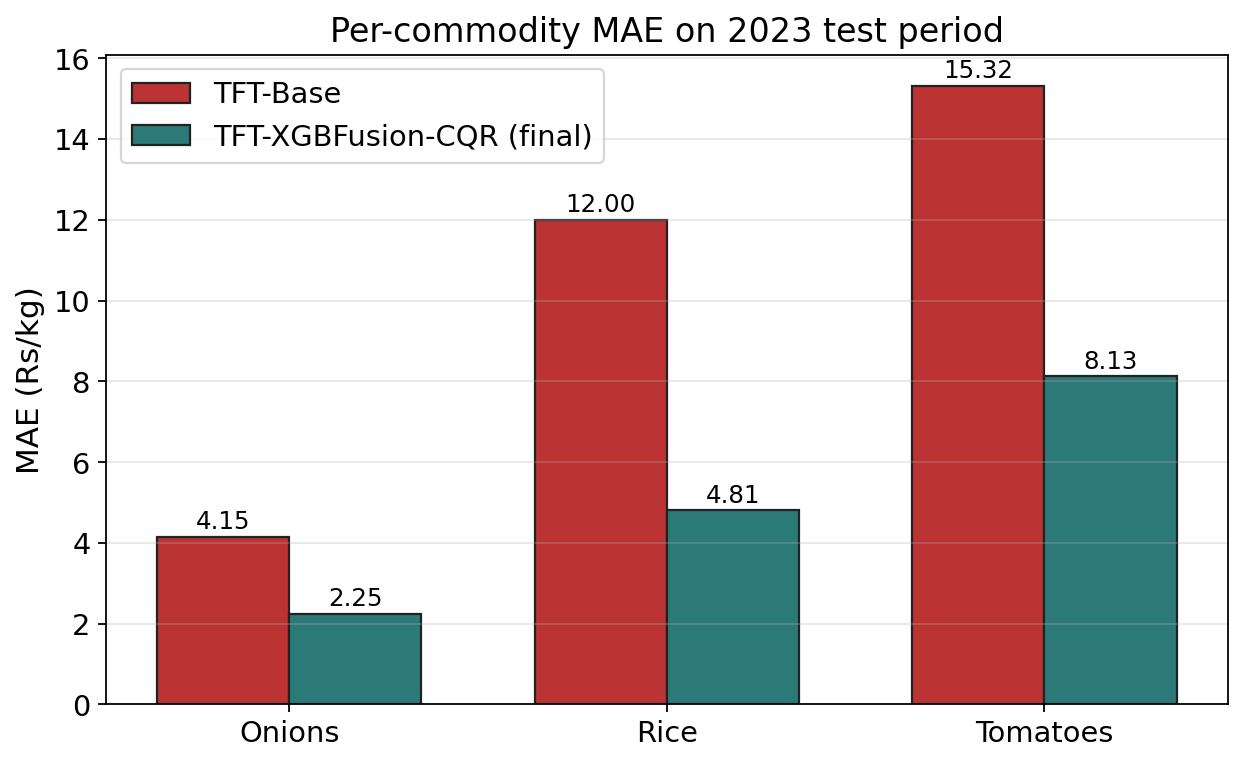
\includegraphics[width=0.95\linewidth]{figures/per_commodity_mae_comparison.png}
\caption{Per-crop MAE on the 2023 test period: plain TFT vs the final fused-and-calibrated model.}
\label{fig:per_commodity_mae}
\end{figure}

Figure~\ref{fig:quantile_forecasts} plots the calibrated prediction band over the actual prices for each crop during the test period. The shaded region is the $q_{0.1}$ to $q_{0.9}$ calibrated band. The solid line is the median forecast. The onion and rice plots track the actual price closely. For tomatoes, the band correctly widens during the mid-2023 price surge, which matches the higher uncertainty in that period.

\begin{figure*}[!t]
\centering
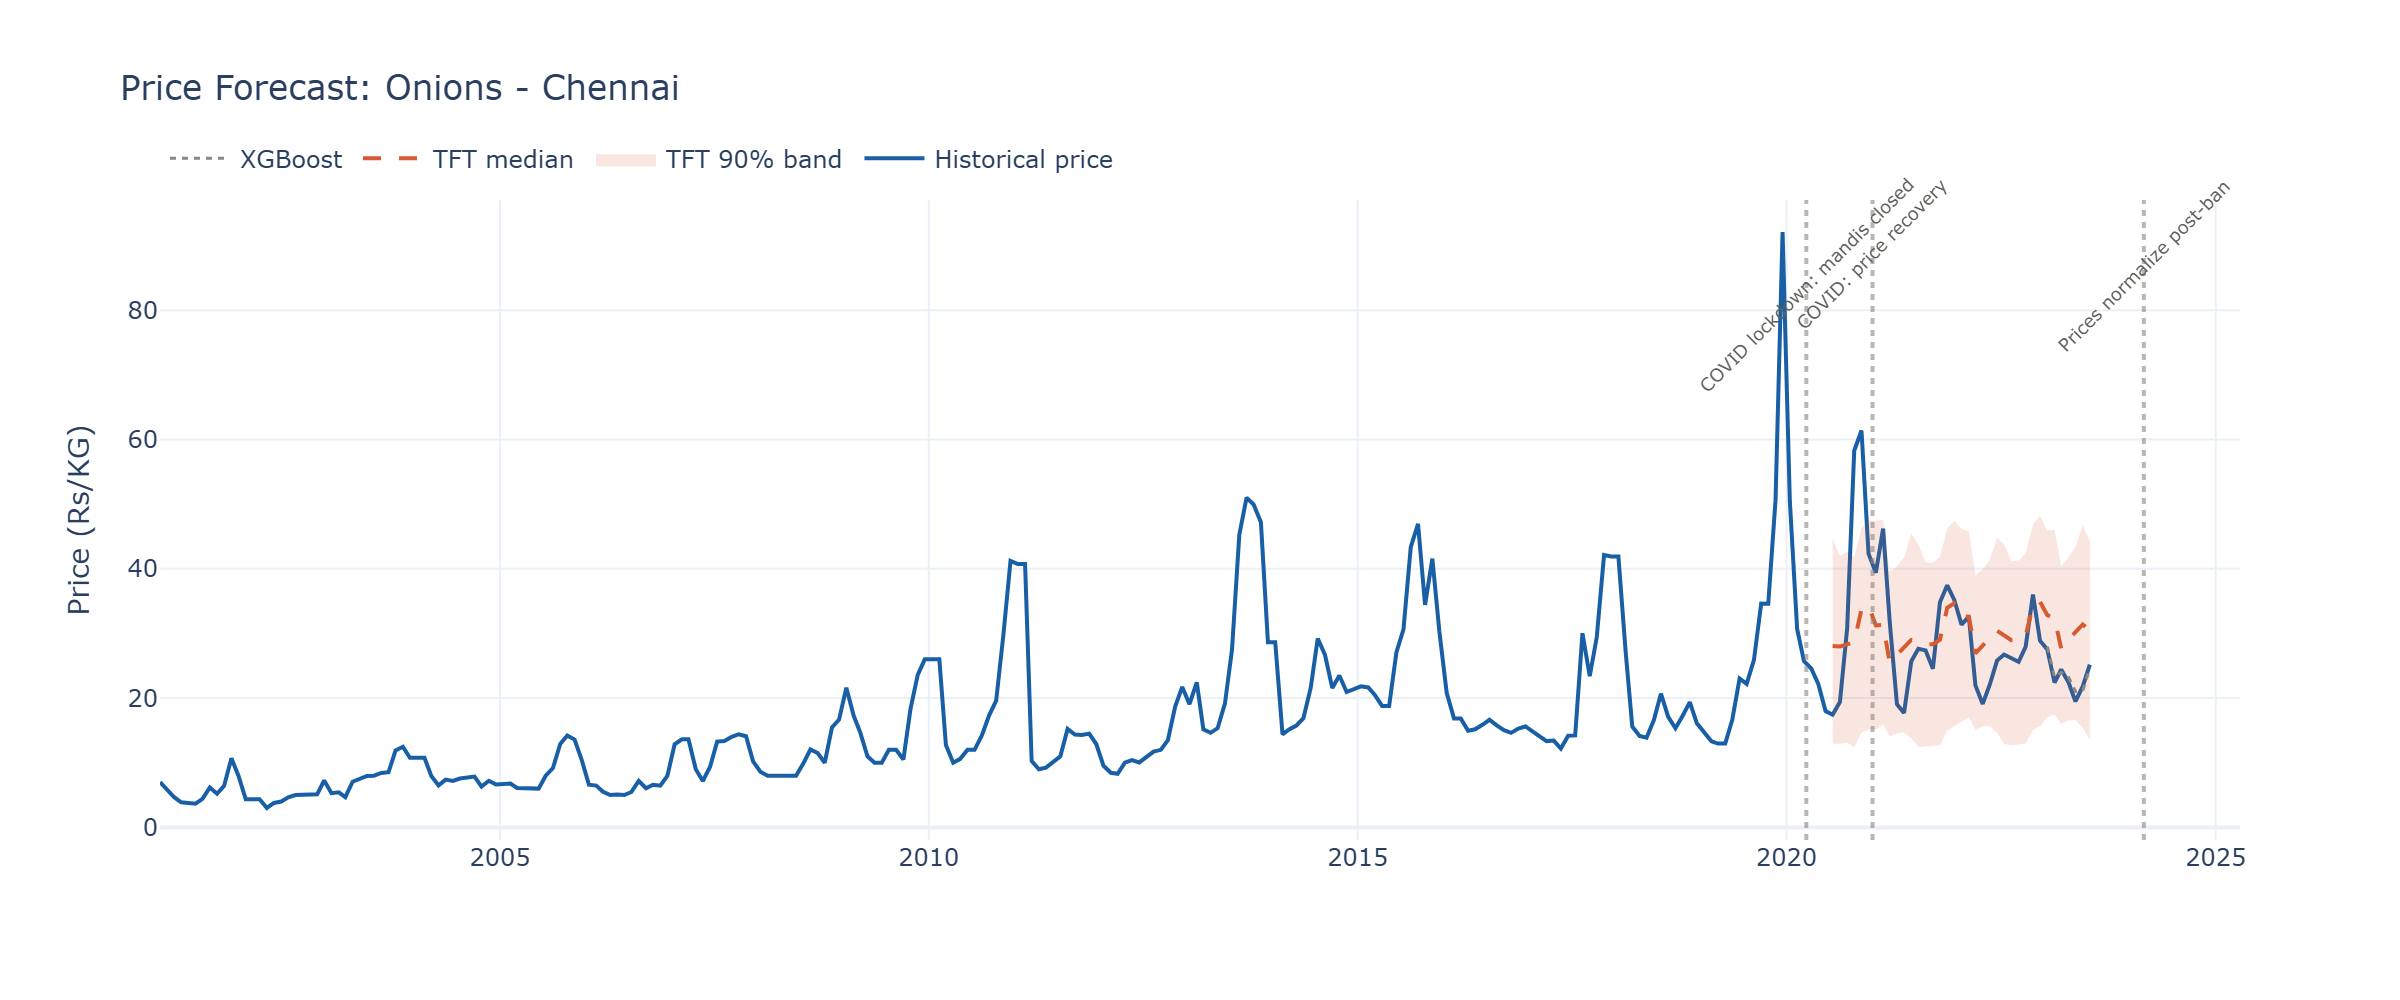
\includegraphics[width=0.95\linewidth]{figures/paper/quantile_forecast_onions.png}\\[3pt]
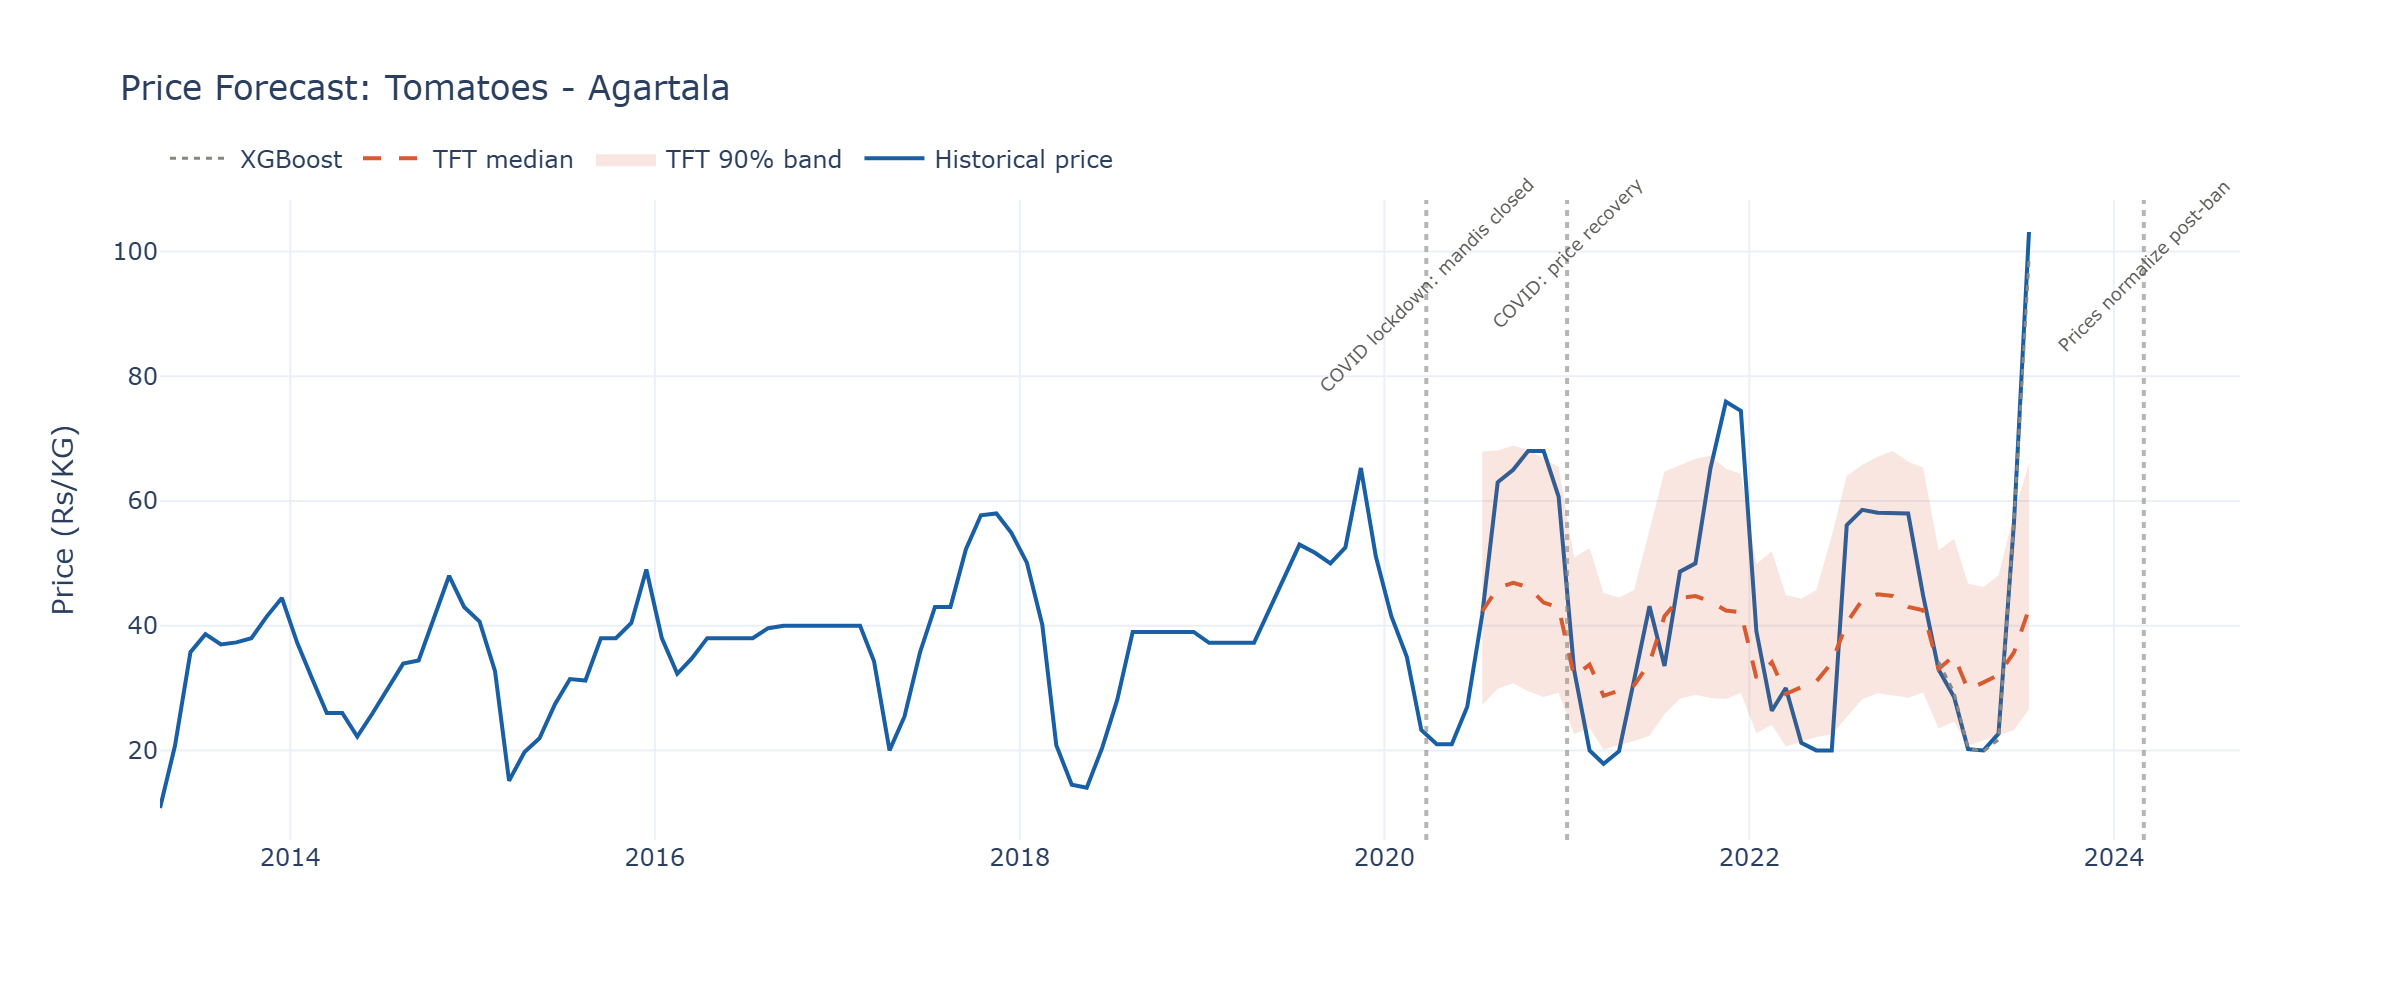
\includegraphics[width=0.95\linewidth]{figures/paper/quantile_forecast_tomatoes.png}\\[3pt]
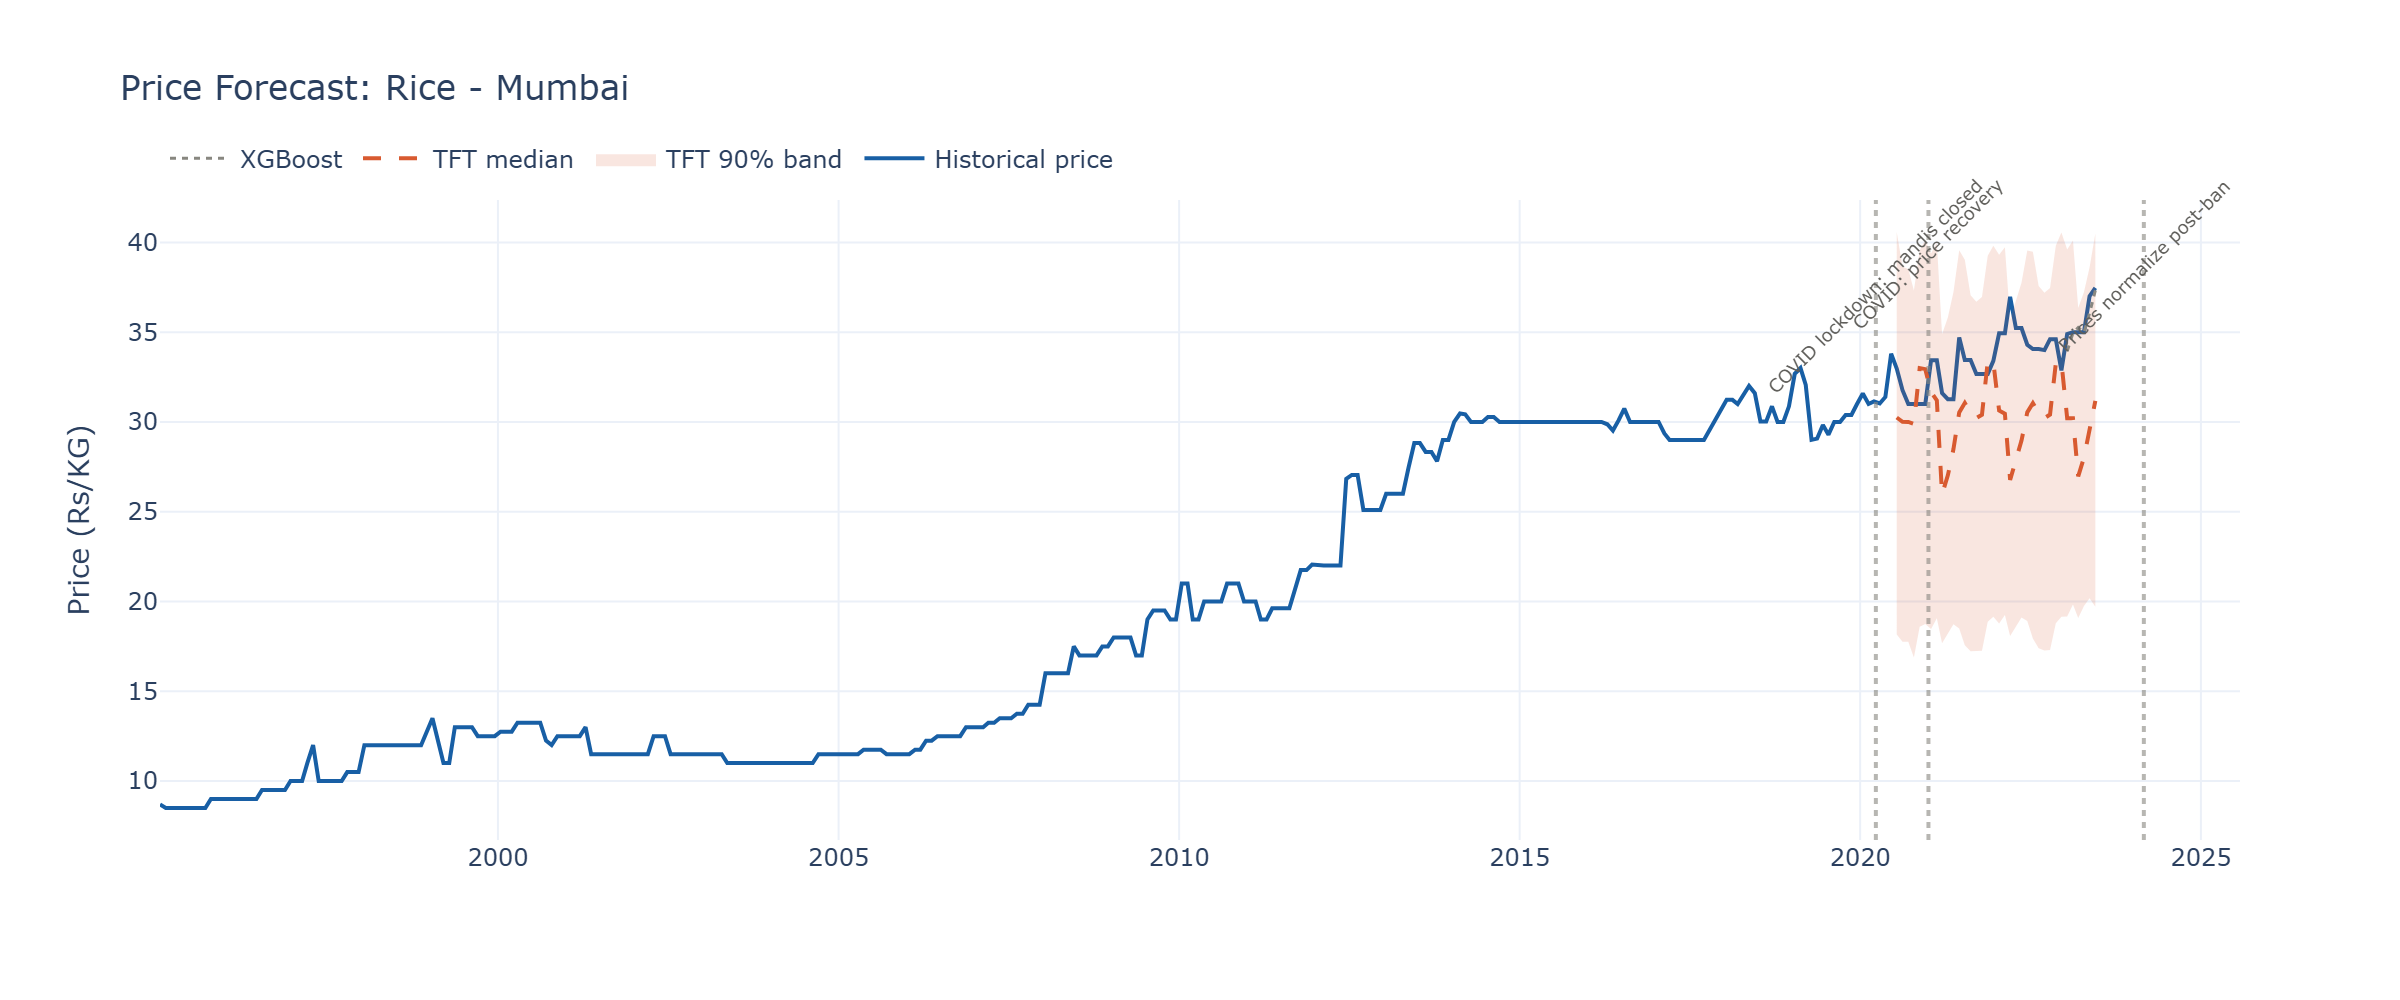
\includegraphics[width=0.95\linewidth]{figures/paper/quantile_forecast_rice.png}
\caption{Calibrated TFT-XGBFusion-CQR prediction band (shaded) and median forecast (solid line) over actual prices for onions (top), tomatoes (middle) and rice (bottom) on the 2023 test set.}
\label{fig:quantile_forecasts}
\end{figure*}

\subsection{Statistical validation of the improvement}
\label{sec:stat_proof}
Three statistical tests were run on the 792 test rows to confirm that the gain over the plain TFT is not due to chance. The same rows are used for both models, so the comparison is fully paired.

\textbf{Paired two-sided $t$-test.} The null hypothesis $H_0$ is that the mean absolute-error difference between the two models is zero. Result: mean MAE reduction = 5.577 Rs per kg, $t = -22.34$, $p = 4.6 \times 10^{-86}$. $H_0$ is rejected. The gain is statistically real.

\textbf{Wilcoxon signed-rank test.} The $t$-test assumes the error differences are roughly normal. The Wilcoxon test does not. It works on the ranks of the differences and acts as a non-parametric backup. Result: $p = 1.2 \times 10^{-95}$. Both tests agree.

\textbf{Cohen's $d$ effect size.} At large $n$, a tiny improvement can still be statistically significant. Cohen's $d$ measures the standardised gap between the two error distributions. A value above $|d| = 0.5$ counts as large. Result: $d = -0.79$. The gain is large in practical terms, not just statistical.

Table~\ref{tab:stat_tests} summarises the three tests for the key comparison.

\begin{table}[H]
\centering
\caption{Paired ablation tests on $n = 792$ matched market-date rows from the 2023 test period. Cohen's $|d| > 0.5$ indicates a large practical effect.}
\label{tab:stat_tests}
\begin{tabular}{lc}
\toprule
\textbf{Statistic} & \textbf{Fusion vs TFT-Base} \\
\midrule
$\Delta$MAE (Rs per kg) & $-5.577$ \\
$t$                 & $-22.34$ \\
$p$ (paired $t$)    & $4.6 \times 10^{-86}$ \\
Wilcoxon $p$        & $1.2 \times 10^{-95}$ \\
Cohen's $d$         & $-0.79$ \\
\bottomrule
\end{tabular}
\end{table}

\textbf{Empirical coverage binomial test.} For each crop, an exact two-sided binomial test checks whether the count of test points inside the calibrated band is consistent with the 80 percent nominal target. Table~\ref{tab:coverage_test} lists the results. Rice ($p = 0.695$) and tomatoes ($p = 0.310$) match the 80 percent target. Onions over-cover at 90.9 percent ($p < 0.001$). The band is therefore wider than needed for onions. Given the onion price spike history, a wider band is acceptable.

\begin{table}[H]
\centering
\caption{Per-crop binomial test of empirical coverage. $H_0$: empirical coverage $= 80\%$ (nominal). $p > 0.05$ means statistically consistent with nominal.}
\label{tab:coverage_test}
\begin{tabular}{lcccc}
\toprule
\textbf{Crop} & \textbf{$n$} & \textbf{Hits} & \textbf{Coverage} & \textbf{$p$} \\
\midrule
Onions   & 242 & 220 & 90.9\% & $<0.001$ \\
Tomatoes & 297 & 245 & 82.5\% & 0.310 \\
Rice     & 253 & 200 & 79.1\% & 0.695 \\
\textbf{All} & \textbf{792} & \textbf{665} & \textbf{84.0\%} & \textbf{0.005} \\
\bottomrule
\end{tabular}
\end{table}

\begin{figure}[H]
\centering
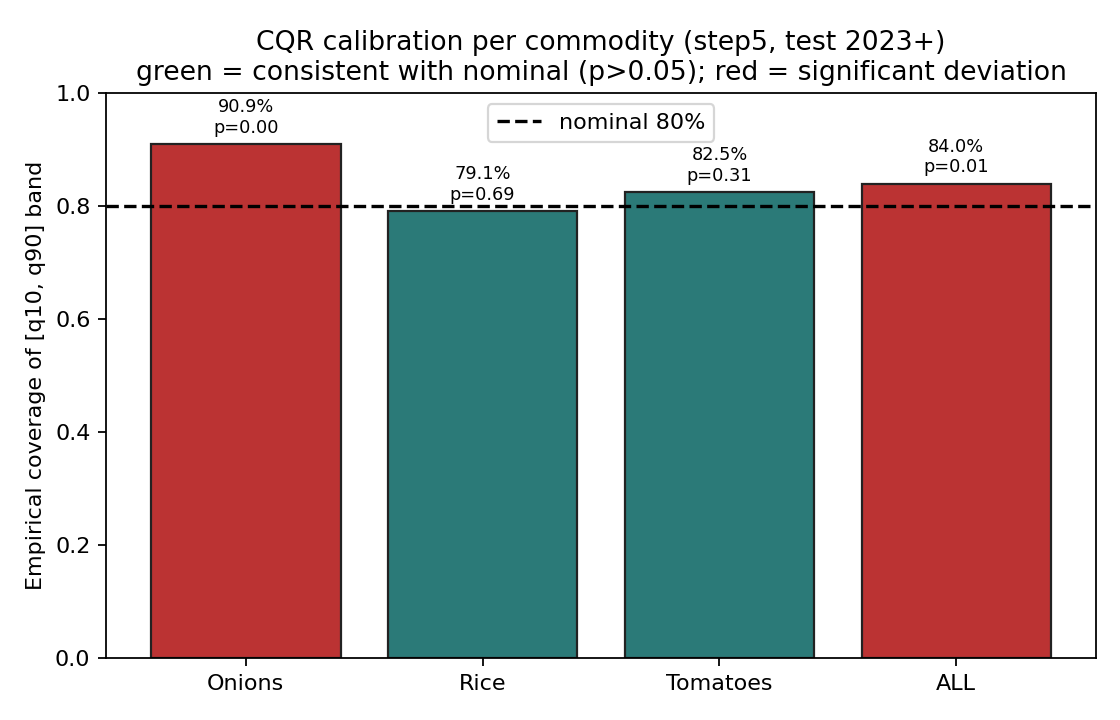
\includegraphics[width=0.85\linewidth]{figures/coverage_plot.png}
\caption{Empirical coverage of the calibrated 80 percent prediction band by crop on the 2023 test set. The dashed line is the nominal 80 percent target. Bars statistically consistent with nominal ($p > 0.05$) are shown in green.}
\label{fig:coverage_plot}
\end{figure}

\textbf{VSN bootstrap stability.} An explanation is only useful if it is reproducible. To check the stability of TFT's feature ranking, 1000 random resamples of market-crop series are drawn with replacement. Each resample gives a feature ranking from the VSN encoder weights. Pairwise Kendall rank correlations are then computed across all resampled rankings. A $\tau$ value close to 1 means the rankings are nearly identical across resamples. A value close to 0 means the rankings are random. Result: \textbf{mean $\tau = 0.942$, 95 percent confidence interval $[0.895,\ 0.990]$}. The ranking is highly stable.

The top features fall into three groups. Weather sits at the top: mean temperature (0.143), excess rainfall (0.143) and deficit rainfall (0.140), followed by humidity (0.066). Calendar and event variables come next: year (0.060), the COVID lockdown flag (0.059) and the agricultural season (0.042). Price-memory features round out the top ten: log price (0.041), the six-month rolling mean (0.038) and the twelve-month price lag (0.038). The ordering matches what a domain expert would expect. Weather drives supply. The season and event flags handle structural shifts. Price memory carries the short-term momentum.

\begin{figure}[H]
\centering
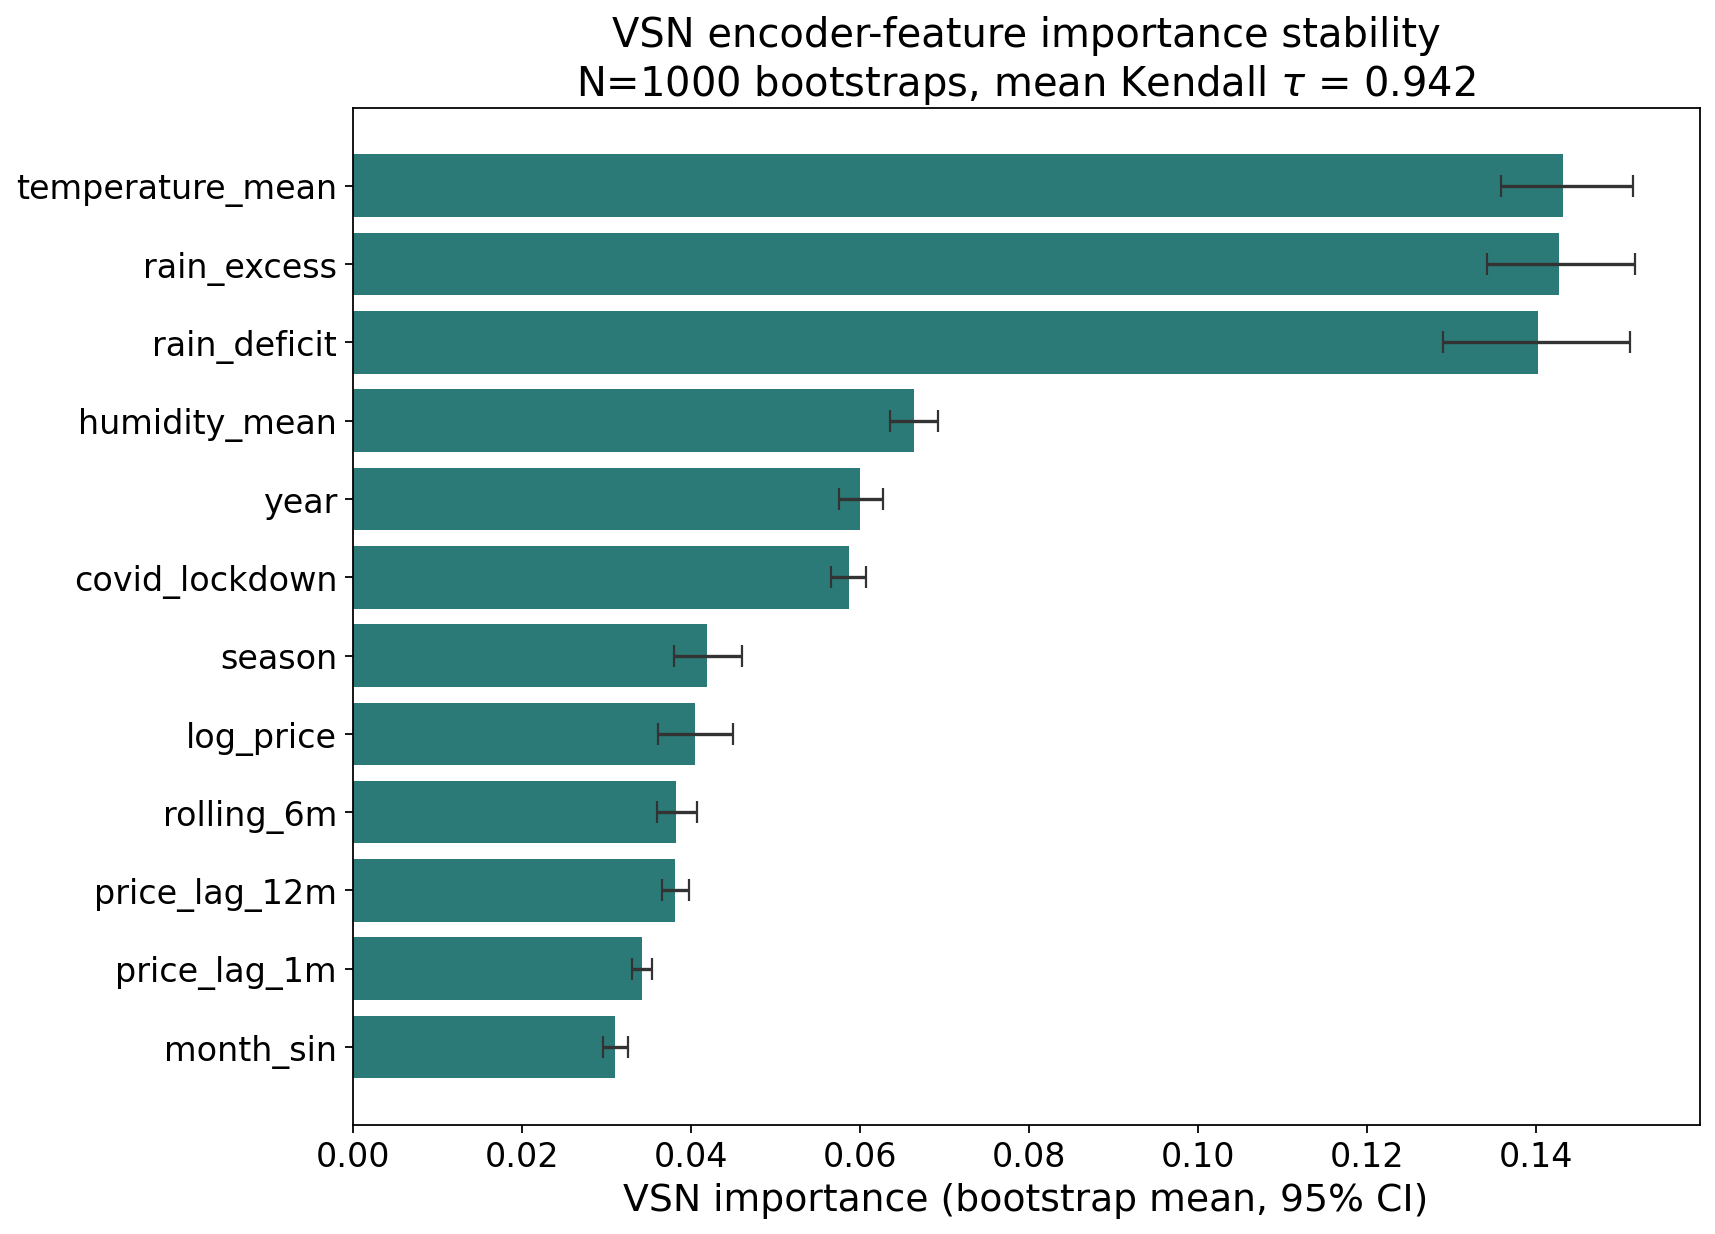
\includegraphics[width=0.95\linewidth]{figures/vsn_bootstrap_stability.png}
\caption{Top TFT encoder features ranked by bootstrap-mean VSN importance with 95 percent confidence intervals (1000 resamples). Kendall $\tau = 0.942$ confirms the ranking is stable across resamples.}
\label{fig:vsn_stability}
\end{figure}

\begin{figure}[H]
\centering
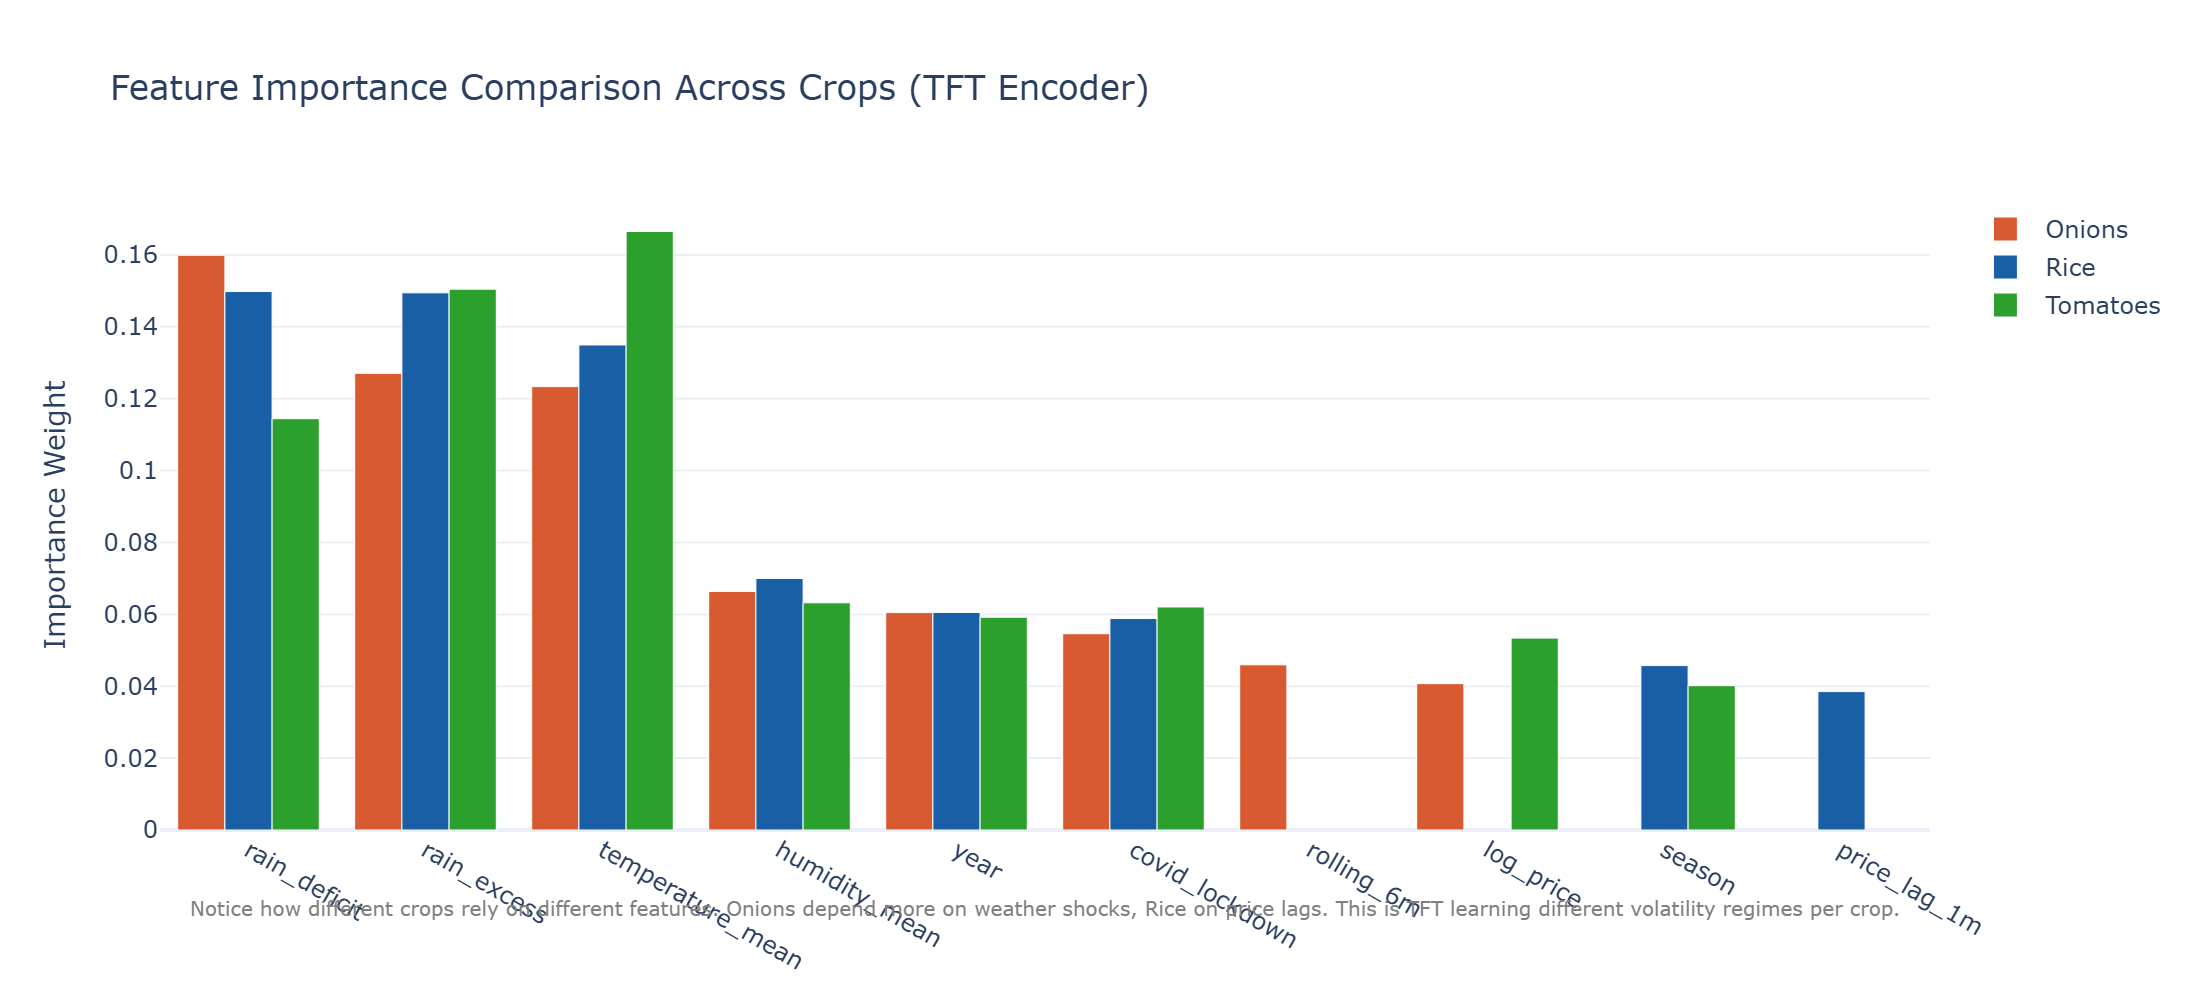
\includegraphics[width=0.85\linewidth]{figures/paper/variable_importance_comparison.png}
\caption{Comparison of encoder and decoder VSN feature importances. Weather and price-memory features dominate consistently across both the encoder and decoder pathways.}
\label{fig:varimp_comparison}
\end{figure}

A high VSN weight on rain deficit means the trained model relies on that variable heavily during prediction. It does not prove that a rainfall deficit caused the price move. The point is auditability. The attribution patterns are stable and domain-consistent, so each forecast can be checked by a domain expert.

\subsection{Comparison with prior work}
Table~\ref{tab:lit_compare} gives an indicative comparison with prior Indian crop price forecasting studies. Direct numerical comparison is difficult because each study uses different crops, markets, time periods and prediction frequencies. Monthly data smooths within-month spikes that daily or weekly models must absorb, so monthly MAPE values are naturally lower than daily MAPE values.

\begin{table*}[!t]
\centering
\caption{Indicative comparison with prior Indian crop price forecasting work. MAPE values are not directly comparable across studies due to differences in crops, markets and update frequencies.}
\label{tab:lit_compare}
\begin{tabular}{p{4.5cm}p{4.0cm}p{1.5cm}p{5.0cm}}
\toprule
\textbf{Work} & \textbf{Crops} & \textbf{MAPE} & \textbf{Reports uncertainty?} \\
\midrule
Nayak et al.\ \cite{nayak2024top}        & Tomato, Onion, Potato  & 8--15\% & no \\
Manogna et al.\ \cite{manogna2025deep}   & Multiple crops         & 5--20\% & no \\
Paul et al.\ \cite{paul2022brinjal}      & Brinjal                & 7--12\% & no \\
\textbf{This work}                       & Onions, Tomatoes, Rice & \textbf{11.4\%} & \textbf{yes (84\% coverage)} \\
\bottomrule
\end{tabular}
\end{table*}

XGBoost on its own gives the lowest point MAPE because tree ensembles are very effective on engineered tabular features. It does not produce a calibrated band or per-timestep explanation. The fused and calibrated model gives the strongest combined result: a competitive MAPE of 11.4 percent, an empirically valid band at 84 percent coverage with an average width of around 12 Rs per kg, and a feature ranking that is stable across 1000 bootstrap resamples. For market monitoring, where an overconfident or underconfident forecast can lead to poor procurement or storage calls, this combined behaviour is more valuable than the lowest point error alone.

%% =====================================================================
%% SECTION 8 — IMPLEMENTATION AND DASHBOARD
%% =====================================================================
\section{Implementation and Dashboard}
\label{sec:implementation}

The trained artifacts --- the XGBoost model file, the TFT checkpoint and the per-crop CQR offsets --- are loaded into a Streamlit application. The application has four views for any chosen crop and market. The active model is selected at startup based on the artifacts present, so the dashboard always runs the best available model.

Figure~\ref{fig:dash_main} shows the main view, which is the one used for actual decision making. For each month from one to six ahead, the view shows the median predicted price, the lower and upper bounds of the calibrated band, and a risk label. The risk label is derived from the relative band width and takes three values: stable, uncertain or high risk. Two months may have similar median forecasts but very different bands. That difference matters for a trader or a procurement planner. The other three views support the same workflow. A price-tracking view overlays the actual price with XGBoost, the TFT median and the calibrated band. An explainability view shows XGBoost gain values, TFT VSN weights and temporal attention. A test-validation view overlays the actual prices on the 2023 test period so the model can be audited on data it never saw. The artifacts are loaded once at startup. The historical panel is read from processed CSV files. This keeps the prototype lightweight and self-contained.

\begin{figure}[H]
\centering
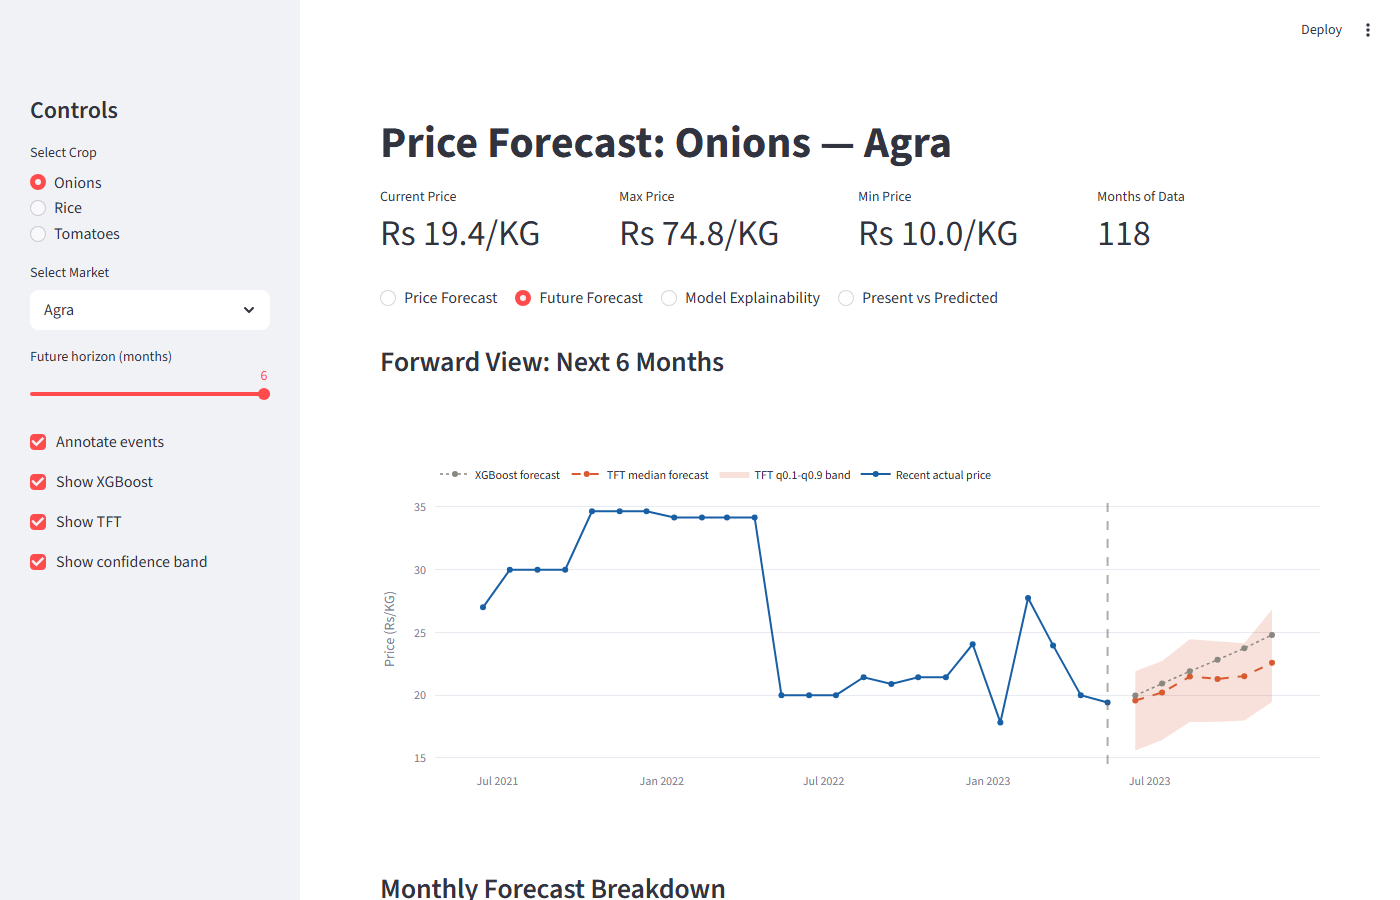
\includegraphics[width=\linewidth]{figures/dashboard_view2_future.png}
\caption{Future forecast view of the dashboard. For each of the next one to six months the system shows the median predicted price, the calibrated band, and a risk label derived from the relative band width.}
\label{fig:dash_main}
\end{figure}

%% =====================================================================
%% SECTION 9 — CONCLUSION AND FUTURE WORK
%% =====================================================================
\section{Conclusion and Future Work}
\label{sec:conclusion}

This paper has presented a crop price forecasting setup that combines a gradient boosted point predictor (XGBoost), a probabilistic deep model with built-in interpretability (TFT), feature fusion between the two, and per-crop CQR calibration. On the 2023 test period for onions, tomatoes and rice across 123 market-crop series, the final model reaches 11.4 percent MAPE and 84.0 percent empirical coverage for the calibrated 80 percent band, with an average width of around 12 Rs per kg. Three statistical tests back this result: a paired $t$-test gives $p = 4.6 \times 10^{-86}$, a Wilcoxon test gives $p = 1.2 \times 10^{-95}$, and Cohen's $d = -0.79$ indicates a large practical effect size. The feature ranking is stable across 1000 bootstrap resamples (Kendall $\tau = 0.942$).

One trade-off is worth stating directly. XGBoost on its own achieves a lower point MAPE (2.8 percent) than the fused probabilistic model, but it produces no band, no confidence measure and no per-timestep explanation. The contribution of this work is the combined system that produces all three, exposed through a usable dashboard.

Several limitations are worth noting. All inputs and targets are monthly aggregates. A one-week heat shock in June can push tomato prices by 50 percent in that month's retail cycle, yet the model sees only the monthly average temperature --- the shock is invisible. The test window runs from January 2023 to July 2023, roughly seven months. While the statistics over 792 rows are reliable, a longer test period covering another full seasonal cycle would strengthen the conclusions. The dashboard loads fixed artifacts and does not pull fresh data automatically; it is a prototype, not a monitoring system.

The most useful extension would be finer temporal resolution. Weekly mandi arrival and price data from Agmarknet would let the model respond to within-month supply shocks rather than seeing them only after they have averaged out. On the input side, the current feature set is limited to weather and price history. News-derived signals --- procurement announcements, transport strikes, export bans --- often move before the price series does. The CQR calibration offsets are fixed at 2022 values. If the underlying price regime shifts structurally, as it did during COVID or the 2019 onion crisis, the empirical coverage will drift away from the nominal target. A periodic recalibration step tied to incoming WFP updates would address this. Extending beyond the three crops studied here --- to pulses, potato and edible oils --- would test whether the fusion-plus-calibration design generalises across commodities with different volatility profiles and different levels of government price support.

%% =====================================================================
%% BIBLIOGRAPHY
%% =====================================================================
\bibliographystyle{IEEEtran}
\bibliography{bibliography}

\end{document}
